\section{Velocity Controller}\label{sec:velocityController}
The purpose of the velocity controller is to keep the vehicle at a steady velocity. The PID-controller is the most commonly used - proportional integral differential controller. Often all 3 components are not needed to control the system. Different approaches are explored in the following, starting with the proportional controller.

\subsection{P-Controller}
As seen on \figref{proportionalController} the P-controller is simply a proportional gain which is multiplied in the direct term.
%
\begin{figure}[H]
 	\centering
 	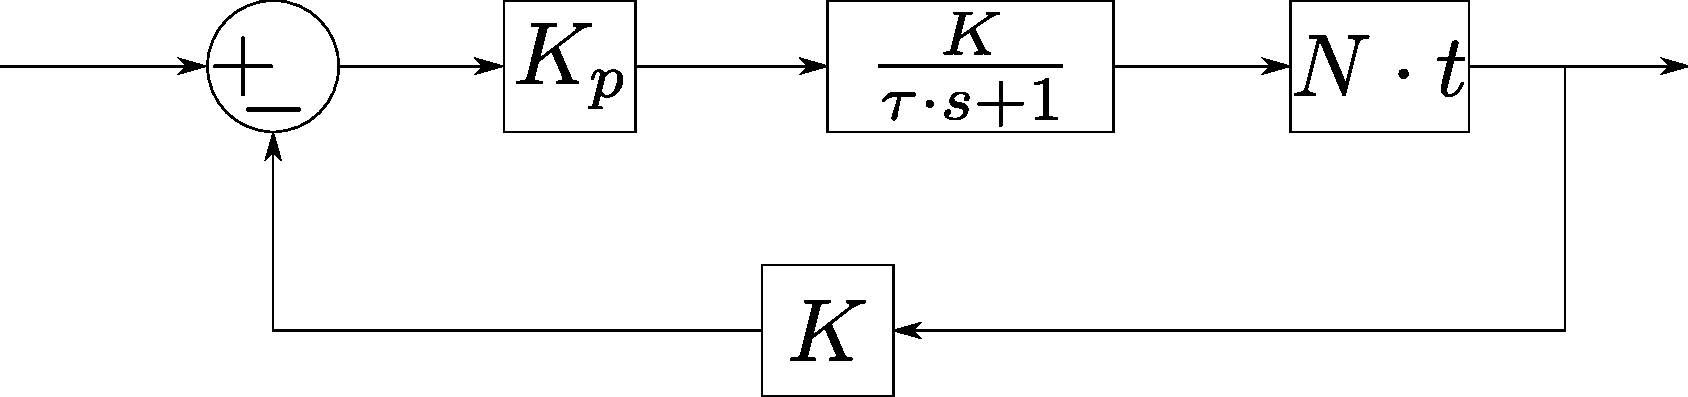
\includegraphics[scale=0.4]{figures/proportionalController.pdf}
 	\caption{Diagram of the proportional controller}
  \label{proportionalController}
\end{figure}
This gives the following closed loop transfer function:
%
\begin{flalign}
  \eq{ \frac{V_{out}}{V_{ref}} }{ \frac{\frac{ K_p \cdot K }{ K_p \cdot K + 1 } }{ \frac{ \tau }{ K_p \cdot K + 1 } \cdot s + 1} }&\label{eq:PclosedLoopTfs}
\end{flalign}
%
From this it is evident that the new system time constant is dependent on the chosen \si{K_p}. The relation is seen directly in the standard form as the coefficient of s:
%
\begin{flalign}
  \eq{ \tau_{closed} }{ \frac{ \tau }{ K_p \cdot K + 1 } }&\nonumber
\end{flalign}
%
So if \si{K_p} is chosen such that it cancels out the gain \si{K} of the plant, allowing for the linear velocity as the input, the time constant will be reduced to half, as will the gain:
\begin{flalign}
  \eq{ \frac{V_{out}}{V_{ref}} }{ \frac{\frac{ \frac{1}{K} \cdot K }{ \frac{1}{K} \cdot K + 1 } }{ \frac{ \tau }{ \frac{1}{K} \cdot K + 1 } \cdot s + 1} }&\nonumber\\
  \eq{ \frac{V_{out}}{V_{ref}} }{\frac{\frac{1}{2}}{\frac{\tau}{2} \cdot s + 1}}&\label{eq:PclosedLoop}
\end{flalign}
%
This means that the P-controller will give an output of half the input, but rise to its set-point twice as fast as the system step without control. This is tested on the vehicle and the response is as expected as seen in \appref{app:proportionalControllerTest}.
%
\subsection{P-Controller with Feed Forward}
Because of its offset the P-controller is not sufficient for reaching and so controlling the decried output velocity. However the P-controller can be improved by manipulating its set-point through use of feed forward, see \figref{proportionalControllerWithFeedforward}.
%
\begin{figure}[H]
 	\centering
 	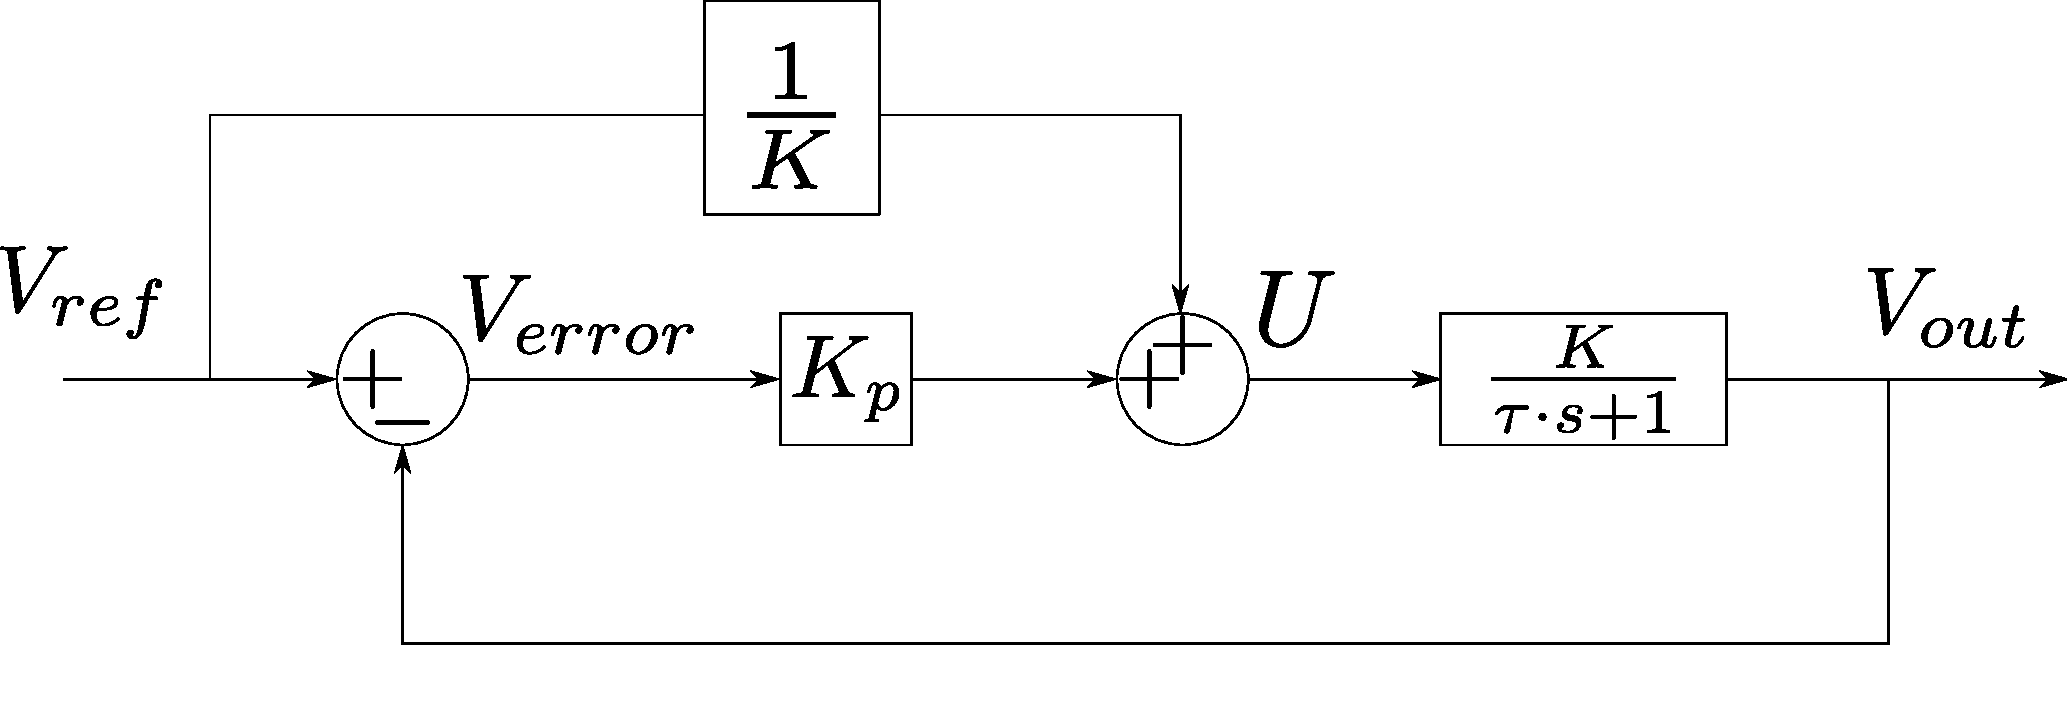
\includegraphics[scale=0.4]{figures/proportionalControllerWithFeedforward.pdf}
 	\caption{Diagram of the proportional controller with feedforward}
 	\label{proportionalControllerWithFeedforward}
\end{figure}
%
In this design the set-point is changed by forward feeding the desired value of the output \si{V_{ref}} to the input of the plant, summing up with the error fed through the P-controller. The gain on the feed forward makes sure that the value of \si{V_{ref}} is in the same unit as the signal going into the plant, here in volts, \si{U}. Since the system gain \si{K} converts volts into linear velocity, the gain in the forward feed is set to \si{\frac{1}{K}}, which yields the following closed loop transfer function:
%
\begin{flalign}
  \eq{ \frac{V_{out} }{V_{ref}} }{ \frac{\frac{K\cdot \frac{1}{K}+K\cdot K_p}{1+K \cdot K_p}}{\frac{\tau}{1+K\cdot K_p}\cdot s + 1 } }&\nonumber
\end{flalign}
%
If the \si{K_p} value again is selected to cancel out the system gain, allowing for velocity directly on the controller input, the following emerges from the closed loop transfer function:
%
\begin{flalign}
  \eq{ \frac{V_{out} }{V_{ref}} }{ \frac{\frac{K\cdot \frac{1}{K}+K\cdot \frac{1}{K}}{1+K \cdot \frac{1}{K}}}{\frac{\tau}{1+K\cdot \frac{1}{K}}\cdot s + 1 } }&\nonumber\\
  \eq{ \frac{V_{out} }{V_{ref}} }{ \frac{1}{\frac{\tau}{2} \cdot s + 1} }&\nonumber
\end{flalign}
%
If this is compared to the resulting closed loop transfer function for the original P-controller, \eqref{eq:PclosedLoop}, it is immediately obvious that the gain-problem has been solved. Notice that the time constant of the closed loop remains half of that of the plant. So by using the forward feed to place the set-point of the controller, P-control suddenly becomes a viable option for controlling the velocity. This is tested on the vehicle and the response is as expected as seen in \appref{app:proportionalControllerTest}. Comparing the step response with the simulation of the step, see figure \figref{fig:stepPfeedForward}, there are a few thing to notice.
%
\begin{figure}[H]
 	\centering
 	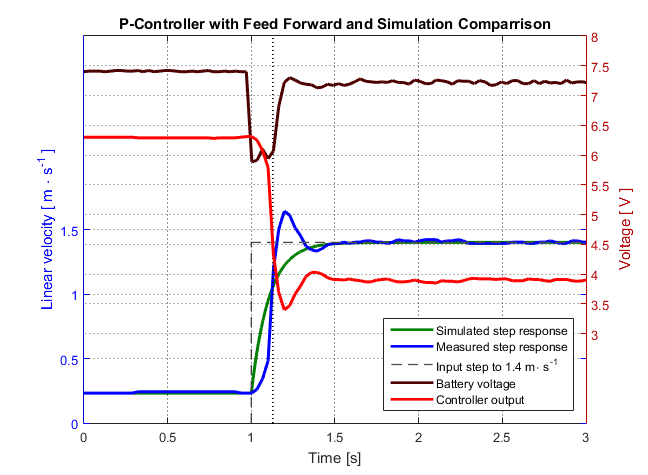
\includegraphics[width=.8\textwidth]{figures/stepPfeedForward}
 	\caption{Proportional control with feed forward. The simulation is first order while the vehicle is second order due to the armature coils in the motor.}
 	\label{fig:stepPfeedForward}
\end{figure}
%
First, the rise time of the two are approximately equal, however, the simulation of the first order approximation rises directly, while the measured data has a delayed initial rise. This delay is presumably because of the armature coils in the motor, through which the current cannot change instantaneously. This effect gives rise to a second order term, as discussed in \secref{DriveTrain}, where the first order approximation was made. After the armature coils have been energized the controller output has a much faster effect on the velocity of the vehicle, causing it to rise so fast that it overshoots due to inertia.
An other interesting thing to notice is the sudden drop in battery voltage. When large currents are drawn from a NiMH battery, the voltage drops\cite{BatteryDS}. However in the implementation the duty cycle is scaled according to the current battery voltage, so that the controller maintains the same effect regardless of battery voltage. The exception being when the controller output exceeds the battery voltage, in which case the control will follow the battery voltage until the battery recovers. If the voltage drop at large current draws turn out to be a problem, an option could be to consider LiPO batteries, which are better at keeping a constant voltage, regardless of the amount of current drawn.

The P-controller with feed forward seem to be a good choice, however if subjected to disturbances, some problems emerge. For instance adding friction when breaking, exceeds the capabilities of a feed forward P-controller. The set-point compensation origins at the input of the controller, so when a disturbance is imposes on the system, the gain of the plant suddenly changes, and this cannot be accounted for with this feed forward P-controller. The effect is demonstrated in \figref{fig:hillPfeedForward}, where the controller was tested on a hill.
%
\begin{figure}[H]
 	\centering
 	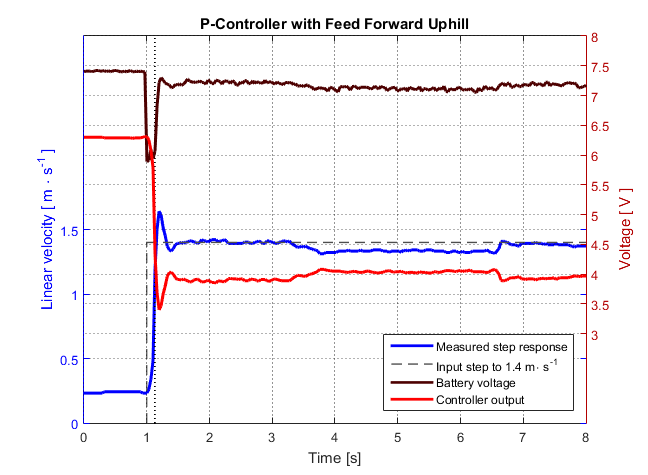
\includegraphics[width=.8\textwidth]{figures/hillPfeedForward}
 	\caption{When the P-controller with feed forward is subjected to constant disturbances, the gain of the system changes and the proportional gain and set-point is no longer sufficient, to avoid steady state error.}
 	\label{fig:hillPfeedForward}
\end{figure}
%
Since the vehicle steers by breaking on one side, this kind of steady state error will not only occur when encountering slopes, but every time the vehicle turns. To find a better solution a proportional integral controller is considered in the following section.
%
\subsection{PI-Controller} \label{sec:PIcalc}
To attack the new offset-problem caused by changes in the system gain when disturbances enter the system, a proportional integral controller is the next natural choice. The reason for choosing a PI-controller is because the I-component integrates over the error. This component therefore increases or decreases over time, and so has an adaptive effect on the system. The design is outlined in \figref{proportionalIntegratorController}
%
\begin{figure}[H]
 	\centering
 	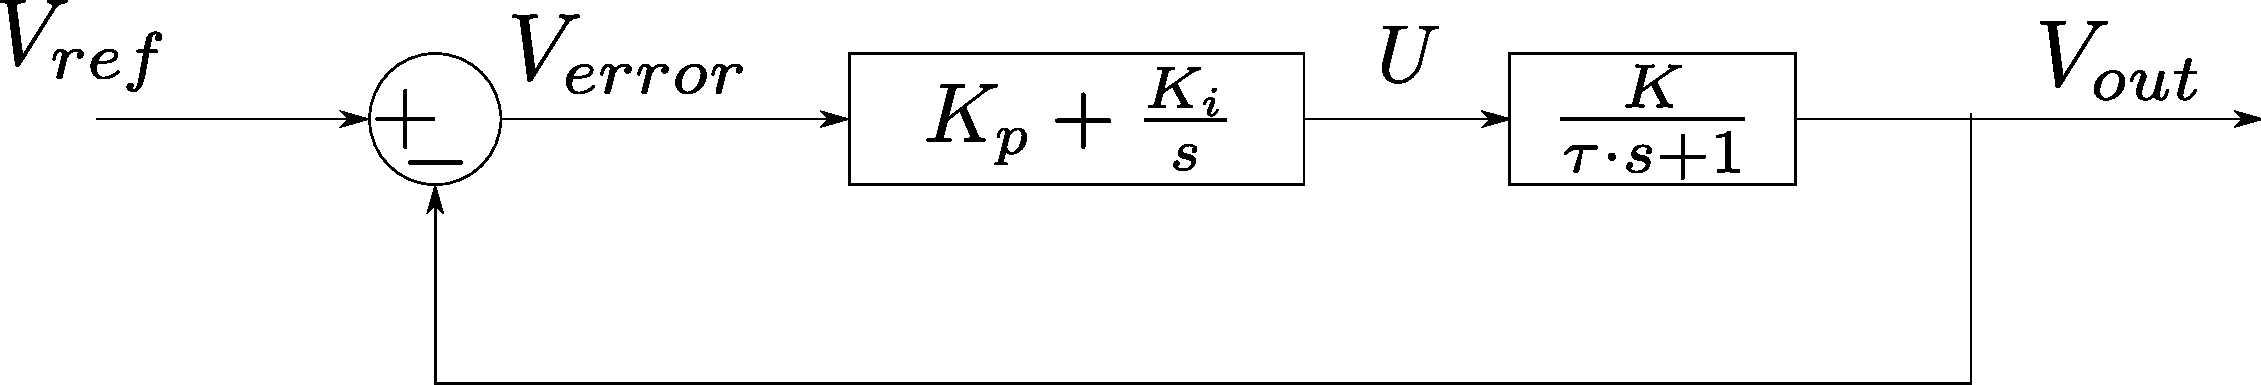
\includegraphics[scale=0.4]{figures/proportionalIntegratorController.pdf}
 	\caption{Diagram of the proportional integral controller}
 	\label{proportionalIntegratorController}
\end{figure}
%
The standard equation for a PI-controller is given and can be rewritten as:
%
\begin{flalign}
  \eq{K_p\cdot(1+ \frac{1}{T_i\cdot s})}{K_p \cdot \frac{T_i \cdot s + 1}{T_i \cdot s}}&\nonumber
\end{flalign}
%
Where \si{T_i} is the time constant of the integrator. Now if the time constant of the integrator is matched to the time constant of the plant, that is \si{T_i = \tau}, the following emerges from the closed loop transfer function:
%
\begin{flalign}
  \eq{\frac{V_{out} }{V_{ref}}}{\frac{K_p \cdot \frac{\tau \cdot s + 1}{\tau \cdot s} \cdot \frac{K}{\tau \cdot s + 1 }}{1 + K_p \cdot \frac{\tau \cdot s + 1}{\tau \cdot s} \cdot \frac{K}{\tau \cdot s + 1 }}}  \ \ \Leftrightarrow  \ \ 
  \si{\frac{V_{out} }{V_{ref}} = \frac{K_p \cdot \frac{K}{\tau \cdot s}}{1 + K_p \cdot \frac{K}{\tau \cdot s} }}&\nonumber
\end{flalign}
%
Inserting \si{K_p = \frac{1}{K}}, yields the following:
%
\begin{flalign}
  \eq{\frac{V_{out} }{V_{ref}}}{\frac{\frac{1}{K} \cdot \frac{K}{\tau \cdot s}}{1 + \frac{1}{K} \cdot \frac{K}{\tau \cdot s} }} \ \ \Leftrightarrow  \ \  \si{\frac{V_{out} }{V_{ref}} = \frac{\frac{1}{\tau \cdot s}}{1 + \frac{1}{\tau \cdot s} }} \ \ \Leftrightarrow  \ \  \si{\frac{V_{out} }{V_{ref}} = \frac{1}{\tau \cdot s + 1}}&\nonumber
\end{flalign}
%
This is equivalent to the plant but with a gain of 1 instead of K, which is desirable, and so also the reason for inserting \si{K_p = \frac{1}{K}}.
Now to determine \si{K_i}, the original equation for a PI-controller is evaluated:
%
\begin{flalign}
  \si{K_p + K_i\cdot \frac{1}{s}} &= \si{K_p\cdot(1+ \frac{1}{T_i\cdot s}) \ \ \Rightarrow \ \ K_i\cdot \frac{1}{s} = \frac{K_p}{T_i\cdot s} \ \ \Rightarrow \ \ K_i = \frac{K_P}{T_i} \ \ \Rightarrow \ \ K_i = \frac{K_p}{\tau}}&\nonumber
\end{flalign}
%
This concludes the initial design of the PI-controller, however, in the following the controller will be analyzed and compared to the other controllers. Implementation and discussion of results follow immediately after.

\subsection{Comparison of the Controllers}
On \figref{fig:ControllerSteps} the different controller designs are simulated being subjected to a velocity step. For comparison the plant is subjected to a voltage step calculated from the velocity step and the gain of the plant, which corresponds to a \si{iK_p}, but without feedback control.
%
\begin{figure}[H]
 	\centering
 	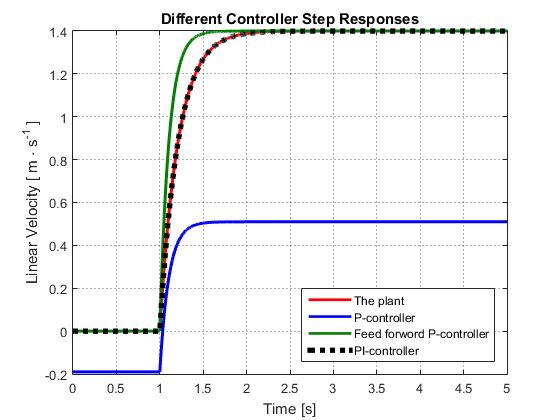
\includegraphics[width=.8\textwidth]{figures/ControllerSteps}
 	\caption{Diagram of the proportional controller}
 	\label{fig:ControllerSteps}
 \end{figure}
%
The first thing to notice on \figref{fig:ControllerSteps}, is the inadequacy of the P-controller, given by its steady state error. The feed forward P-controller however, solving this problem, seems like a very good solution if consulting only its step response. As discussed, a problem arises when introducing a disturbance, as seen in \figref{fig:hillPfeedForward}. The last discussed option is the PI-controller, which places itself right on top of the step response of the plant when having a gain of 1, which is by design. The difference between the plant with a scaled input to obtain a gain of 1, compared to the PI-controller lies in the feedback along with the adaptive gain emerging from the I-component. It becomes clear when investigating the open loop rather than the closed loop transfer function:
%
\begin{flalign}
  V_{error}(s) \cdot \frac{(K_p \cdot \frac{K_i}{s}) \cdot K}{\tau \cdot s + 1}
  \left.\rule{0cm}{1cm}\right\vert\rule{0cm}{.7cm}_{\substack{K_p = \frac{1}{K} \\ \rule{0cm}{.1cm}\\ K_i = \frac{K_p}{\tau}}}
  &\ \ \Rightarrow \ \
  V_{error}(s) \cdot \frac{1}{\tau \cdot s}
  \ \ \xRightarrow{\mathcal{L^{\si{-1}}}} \ \
  \frac{1}{\tau} \cdot \int_{0}^{t} V_{error}(\tau_i) \ d \tau_i &\nonumber
\end{flalign}
%
\hspace{6mm} Where:\\
\begin{tabular}{p{1cm}lll}
  & \si{\tau_i}    & is an integration variable&\\
  & \si{V_{error}} & is the error from \si{V_{ref}-V_{out}}, see \figref{proportionalIntegratorController}&
\end{tabular}

This shows how the integral component of the controller integrates over the error from the reference to the output over time.

On \figref{fig:PIcontrollerStepRealVsSim} a step response of an implemented PI-controller is shown in comparison with the simulated step response with PI-controller.
%
\begin{figure}[H]
 	\centering
 	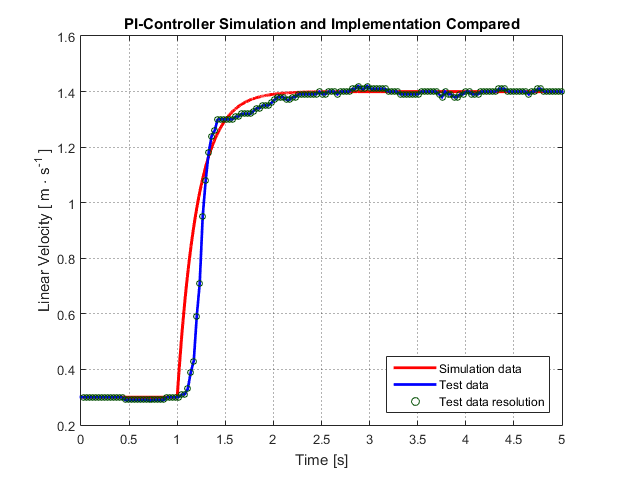
\includegraphics[width=.8\textwidth]{figures/PIcontrollerStepRealVsSim}
 	\caption{Diagram of the proportional integral controller compared to simulation}
 	\label{fig:PIcontrollerStepRealVsSim}
\end{figure}
%
The difference between the two responses at the bottom of the graph might, as mentioned for the feed forward P-controller, be partially due to the fact that the vehicle is a second order system. The approximation to a first order model is however not to be discarded. The design still delivers a response relatively close to the simulation, and as seen from \chapref{cha:AcceptTest}, the PI-controller fulfills the requirements set for the system's velocity controller.
If this implementation is investigated at different velocity steps, a certain characteristic of the current design becomes more apparent, see \figref{fig:multiStepPI}.
%
\begin{figure}[H]
 	\centering
 	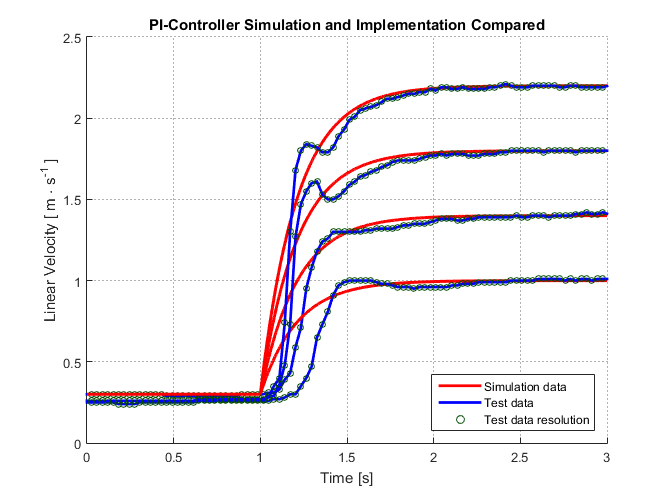
\includegraphics[width=.8\textwidth]{figures/multiStepPI}
 	\caption{Diagram of the proportional controller}
 	\label{fig:multiStepPI}
\end{figure}
%
The system overshoots before reaching the reference velocity. To investigate this behavior further a step is made at 2 \si{m\cdot s^{-1}}, and data from the battery and controller output is recorded, see \figref{fig:PInoAntiWindup}.
%
\begin{figure}[H]
 	\centering
 	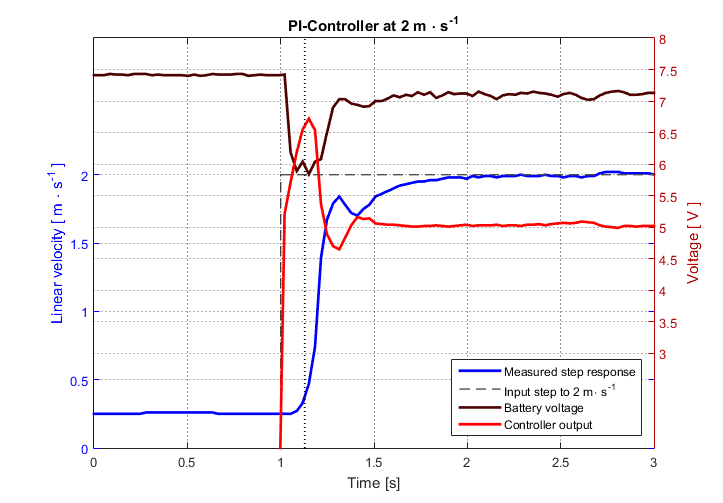
\includegraphics[width=.8\textwidth]{figures/PInoAntiWindup}
 	\caption{Diagram of the proportional controller}
 	\label{fig:PInoAntiWindup}
\end{figure}
%
As mentioned earlier, in this implementation the controller output is converted to duty cycle taking into account a varying battery voltage. So the battery voltage has an impact on the control only when the controller output exceeds the battery voltage. As a side note, the battery voltage is limited to a maximum of \si{100 \ \%} duty cycle.
The overshoot happens after the battery voltage saturation, and so the answer must be found elsewhere.
When the velocity of the vehicle rises, the error naturally falls. The controller output follows this fall of the error. While the integral gain keeps building the \si{V_{error}\cdot K_p} keeps getting smaller due to the rise of the velocity towards the reference. This means that the controller output will keep falling until the integral gain takes over, becoming the most dominant of the two. This is where the controller makes a negative overshoot.
While the controller output was falling beyond its settle value (5 V), the velocity kept going up due to delay cause by inertia in the system. The controller output now rising from the influence of the integral gain, also has a delayed effect on the system.
To conclude, the overshoot of the velocity happening before it reaches its reference is caused by the negative overshoot of the controller output, which originates from the scaling of \si{K_p} and \si{K_i}.
In the following section this overshoot will be further investigated.
%
\subsection{Implementation of the PI controller}
The functional part of the implementation is seen in \autoref{lst:PIimplementation}. The \emph{Actualspeed} is set from the average of recorded speeds of the two belts, from the Hall sensors. Then the error is calculated by comparison between the feedback, \emph{Actualspeed}, and the reference, \emph{Wantedspeed}.
A quick glance at \figref{fig:PInoAntiWindup}, reveals a problem, where the controller output exceeds the battery voltage. This is called empty integral windup, and can be prevented by implementing anti windup, which locks the integral error so that it does not make the controller output voltage exceed the saturation of the battery\todo{source here}. The first if-statement in \autoref{lst:PIimplementation}, is a very simple implementation of an anti-windup functionality, and the effect is clearly demonstrated by repeating the test from \figref{fig:PInoAntiWindup} with anti windup, as seen on figure \figref{fig:PIwithAntiWindup}.

%
\lstset{language=C++, caption={Implementation of the PI-controller}, label=lst:PIimplementation}
\begin{lstlisting}
Actualspeed = (speed0 + speed1)/2; // Average speed of the vehicle

Error = Wantedspeed - Actualspeed;                 //  ANTI-WINDUP:
                                                   //  Only increase integral error if
if( ControllerOutput < ((float)batReading/102.4) ) //<-the battery is not in saturation
{
  Integral = Integral + (Error*0.030); //Delta t = 0.03 s = sample time i.e. 30 ms
}

ControllerOutput = ((Kp * Error) + (Ki * Integral) + Stiction);

DutyPrSpeed = 100.0/((float)batReading/102.4); // Duty cycle pr volt [% pr V]
                                               // batReading/102.4 = volts
Duty = ControllerOutput * DutyPrSpeed;

if(Duty > 100) Duty = 100;  //maximum duty cycle = 100 %
if(Duty < 0) Duty = 0;      //minimum duty cycle =   0 %
\end{lstlisting}
%
\begin{figure}[H]
 	\centering
 	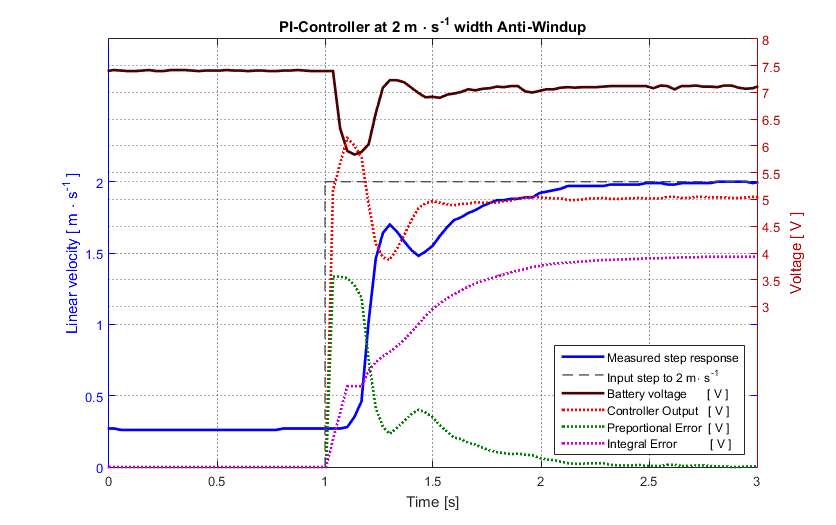
\includegraphics[width=.8\textwidth]{figures/PIwidthAntiWindup}
 	\caption{Diagram of the proportional controller}
 	\label{fig:PIwithAntiWindup}
\end{figure}
%
After making sure that the battery is not in saturation the integral error is increased or decreased depending on weather the error is positive or negative, see line 7 in \autoref{lst:PIimplementaion}. Finally in line 10 the \emph{ControllerOutput} is calculated, including the proportional gain, \si{K_p}, and the integral gain, \si{K_i}, along with the \emph{Stiction}, which is a voltage offset to counter the effect of stiction.
The duty cycle is then calculated in line 12 and 14, where it is scaled according to the current battery voltage, so that each controller output applies the calculated voltage, regardless of the battery voltage. This implementation with the calculated proportional and integral constants, see \secref{sec:PIcalc}, is tested at \si{1.4 m\cdot s^{-1}}, see \figref{fig:CalculatedPI}.
%
\begin{figure}[H]
 	\centering
 	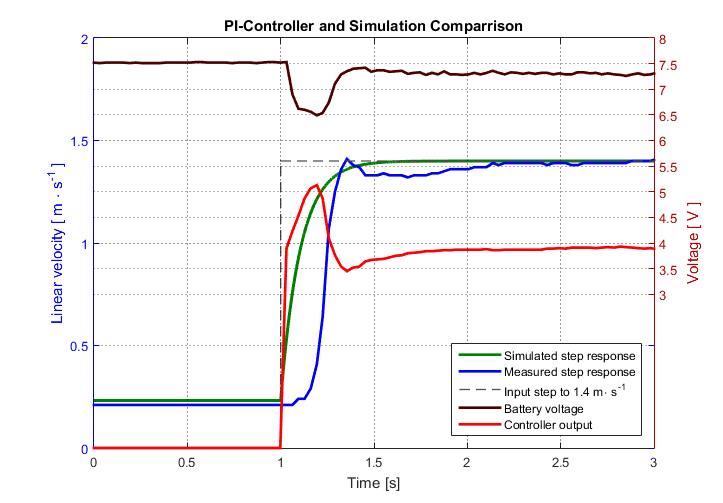
\includegraphics[width=.8\textwidth]{figures/CalculatedPI}
 	\caption{Diagram of the proportional controller}
 	\label{fig:CalculatedPI}
\end{figure}
%
The reality diverges from the simulation as previously mentioned, because it is a first order approximation. The previously addressed controller overshoot, can be minimized by tuning the proportional and integral gain, so that the transition between dominance of the two gains, becomes more smooth at the wanted operation speed, \si{1.4 m\cdot s^{-1}}. The tuning has been done with multiple iterations applying a trial and error approach. The result is shown on \figref{fig:TunedPI}, where the dip in the battery voltage is minimal, due to the longer rise-time, which also minimizes overshoot. 
%
\begin{figure}[H]
 	\centering
 	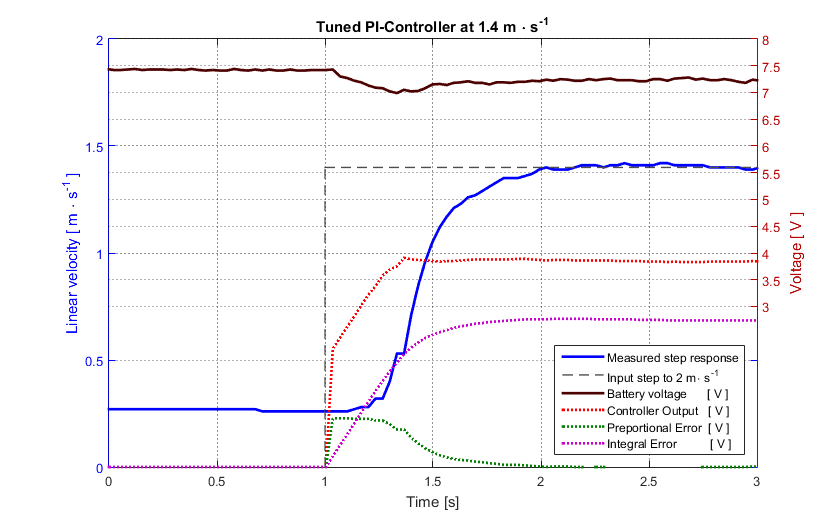
\includegraphics[width=.8\textwidth]{figures/TunedPI}
 	\caption{Diagram of the proportional controller}
 	\label{fig:TunedPI}
\end{figure}
%
The test is carried out on a ramp, which goes up and then flattens out. The same ramp was used for testing the P-controller with feed forward, see \figref{fig:hillPfeedForward}, where a steady state error occurred, while on the hill. Whereas the PI-controller's integral gain closes this steady state error, and so keeps the speed when on the hill.